\documentclass[11pt, a4paper, twocolumn]{article}

% Fonts and math (Elsevier-like Times style)
\usepackage{graphicx} % Required for inserting images
\usepackage{array} % For extra column formatting
\usepackage{amsmath, amssymb, cancel, siunitx, mathtools, physics2, upgreek} % for equation environment
\usepackage{float,geometry,subcaption}
\geometry{margin=2cm}
\usepackage[skip=10pt]{parskip}
\usepackage{setspace}
\usepackage{hyperref, cleveref}
\usepackage{cite, bookmark}
\usepackage{url}
\usepackage[table,xcdraw]{xcolor}
\usepackage[export]{adjustbox}
\usepackage{listings,pdfpages}
\usepackage{dblfloatfix}

% --- Abstract styling (elsarticle look)
\usepackage{abstract}
\renewcommand{\abstractnamefont}{\normalfont\bfseries}
\renewcommand{\abstracttextfont}{\normalfont}
\renewenvironment{abstract}{%
  \par\noindent\rule{\linewidth}{0.4pt}\par
  \begin{center}\bfseries Abstract\end{center}%
}{%
  \par\rule{\linewidth}{0.4pt}\par
}

% --- Section styling (similar to elsarticle
\usepackage{titlesec}
\titleformat{\section}{\normalfont\large\bfseries}{\thesection.}{0.5em}{}
\titleformat{\subsection}{\normalfont\normalsize\bfseries}{\thesubsection.}{0.5em}{}

% Table of contents styling
\usepackage{tocloft}
\cftsetindents{section}{0em}{2em}
\cftsetindents{subsection}{1em}{2em}
\renewcommand\cfttoctitlefont{\hfill\Large\bfseries}
\renewcommand\cftaftertoctitle{\hfill\mbox{}}
\renewcommand\cftfigfont{\footnotesize}
\renewcommand\cftfigpagefont{\footnotesize}
\renewcommand\cftloftitlefont{\large}

\graphicspath{ {./images/} }

\definecolor{blurple}{HTML}{5865F2}
\definecolor{backcolour}{HTML}{272823}

\hypersetup{
    colorlinks=true,
    linkcolor=black,
    urlcolor=black,
    citecolor=blurple,
}

\urlstyle{same}

\DeclareMathOperator{\sinc}{sinc}

\renewcommand{\arraystretch}{1.4}

% Python code export
\lstset{
    language=Python,
    basicstyle=\ttfamily\scriptsize,
    keywordstyle=\color{magenta},       
    commentstyle=\color{gray},        
    stringstyle=\color{teal},  
    showstringspaces=false,
    frame=single,
    breaklines=true,
    numbers=left,
    numberstyle=\tiny\color{gray}
}

\setcounter{secnumdepth}{5}
\setcounter{tocdepth}{5}

\hbadness=99999

%%%%%%%%%%%%%%%%%%%%%%%%%%%%%%%%%%%

\title{%


\includegraphics[width=0.2\linewidth]{ucd_brandmark_black.jpg} \vspace{0.5cm}\\

{\Large\bfseries UCD School of Physics}\vspace{1.5cm}\\

{\large PHYC30170 Physics Astronomy and Space Lab I}\\
{\bfseries CCD and Spectroscopy}

}
\author{Joana C.C. Adao \\ \small Student No.: 23311051}
\date{\today}

\begin{document}

% Title page - single column
\onecolumn
\maketitle

% Abstract - single column
\thispagestyle{empty}
\begin{abstract}

This experiment sought to investigate the properties of the Messier 91 (M91) as a barred spiral galaxy and the NN Serpentis (NN Ser) eclipsing binary system using CCD imaging and TESS satellite data. Through the reduction of B, H$\upalpha$, and V filter images, a colour composite RGB image of the M91 was generated, successfully displaying the galaxy's characteristic traits, stellar population, and highlighting its anemic, gas-deficient classification. For the NN Ser, photometry was performed on ground-based data to construct a lightcurve, revealing a sharp and deep eclipsing of the primary white dwarf, and a baseline of approximately \textbf{17.5} for r' calibrated magnitudes. This calculated magnitude was found to be roughly 0.8 times dimmer than the accepted magnitude of 16.7 from the SIMBAD database. Furthermore, analysis of the TESS data revealed an orbital period of approximately 0.13 days when plotted on a Lomb-Scargle periodogram, consistent with theoretical expectations of the post-common envelope binary system (PCEB).

\end{abstract}

\newpage

% Table of Contents - single column
\tableofcontents
\pagenumbering{roman}
\setcounter{page}{2}

\newpage

%%%%%%%%%%%%%%%%%%%%%%%%%%%%%%%%%%%

% Start main content in two columns
\twocolumn
\pagenumbering{arabic}
\setcounter{page}{1}

\section{Introduction} \label{sec:1}

\subsection{Photometry}

Photometry relates the number of counts from a source with the magnitude, a basic principle that's given with \cite{photucd}:

\begin{equation} \label{eq:1}
    m_{\text{std}} = -2.5 \log_{10} F + ZP
\end{equation}

with $m_{\text{std}}$ as the calibrated magnitude of a source in the standard system, $F$ is the background-subtracted counts, 
and $ZP$ is the zeropoint for the image, which is determined with reference stars with fluxes/magnitudes on a standard, calibrated system such
that direct comparisons can be made. \cite{photucd}

\autoref{eq:1} is rearranged to obtain the zeropoint of an image, which can be averaged over $n$ sources for the best estimated of a source's 
zeropoint, \cite{photucd}

\begin{equation} \label{eq:2}
    ZP = m_{\text{std}} + 2.5\log_{10}F
\end{equation}

The signal-to-noise ration (SNR) of an image is a source of uncertainty typical of a CCD that can be used to approximate errors on this
aperture photometry with a simplified form \cite{photucd}:

\begin{equation} \label{eq:3}
    \text{SNR} = \frac{F_{\star}}{\sqrt{F_{\star} + n_{\star} \left( 1 + \frac{n_{\star}}{n_{\text{sky}}} \right) \times (F_{\text{sky}} + R^2)}}
\end{equation}

with $F_{\star}$ as the measured \textbf{source} counts, $F_{\text{sky}}$ as the measured \textbf{background annulus} counts, $n_{\star}$ as
the number of pixels within the \textbf{photometric aperture}, $n_{\text{sky}}$ as the number of pixels within the \textbf{background annulus},
and $R$ as the readout noise of the CCD. \cite{photucd}

\autoref{eq:3} can be converted into an uncertainty for the magnitudes is given with \cite{photucd}:

\begin{equation} \label{eq:4}
    \sigma = 2.5 \log_{10}\left( 1 + \frac{1}{\text{SNR}} \right)
\end{equation}

The SNR, uncertainty on the magnitudes, can be added with the mean zeropoint uncertainties, determined with a standard deviation calculation, to
obtain the total photometric uncertainty. \cite{photucd}

\subsection{Messier 91 (NGC 4548)}

The Messier 91 (M91) object is a prominent barred spiral galaxy situated within the Virgo Cluster. It is classified as an SB(rs)b(A) and as a classic example of an "anemic" (A) galaxy due to its significantly lower neutral hydrogen (HI) content and reduced star formation rates compared to similar isolated galaxies. The gas deficiency observed with some objects in this Cluster, including the M91, are attributed to \textit{ram-pressure stripping} as the galaxy moves through the dense intra-medium of the Cluster, which effectively removes the outer cold gas layers necessary for star formation.
\cite{cayatte1990vla,FrommertKronberg2007,graham1999hubble,koopmann2004halpha}

Additionally, H$\upalpha$ imaging of the M91 has revealed a highly truncated gas disk. Unlike healthy spiral galaxies that have H$\upalpha$ emission that extends across the entire disk, the M91's H$\upalpha$ presence is primarily in the inner regions or at the ends of the prominent bar. This is what is referred to as the \textit{anemic} behaviour of a galaxy. \cite{koopmann2004halpha}

\subsection{NN Serpentis}

The NN Serpentis (NN Ser) is a well-studied and recognised post-common envelope binary (PCEB), a low-mass binary system with a hot white dwarf primary and a cool M red dwarf secondary. The system was identified as a pre-cataclysmic eclipsing binary with a short orbital period of approximately \textbf{0.13 days}, or 3.12 hours, making it useful for the study of binary evolution and the physics of the common-envelope phase. \cite{parsons2010precise,beuermann2010two}

\section{Methodology} \label{sec:2}

To analyse the images (provided as FITS files), they \textit{raw} images first be reduced for both the M91 and NN Ser. This is done by first combining the bias images into a masterbias. The masterbias is subtracted from each individual flat field and by combining these subtracted flats, a masterbias is created for each filter (B, V, and H$\upalpha$ for the M91, clear for the NN Ser). The masterflat images can then be normalised by dividing the masterflat by the \textit{averaged} masterflat, which should result in a value of approximately 1. To facilitate future code and avoid errors, the following numpy function can be used:

\;\verb|>> np.clip(normflat, 1e-6, None)|

This clips any value smaller than $\num{1e-6}$ without an upper limit and ensures no future errors when dividing or using a logarithmic fucntion. The creation of a masterbias and normalised masterflat was done for both the M91 and NN Ser objects.

\subsection{Messier 91 (M91)}
\subsubsection{Image Reduction} \label{sec:2.1.1}

To ease repetitive calculations, a function for reducing the images can be made:

\begin{lstlisting}
def deeper_analysis(objfile, masterbias, normalised_flat):
    obj_list = []
    
    for f in objfile:
        objdata = fits.getdata(f).astype(float)
        corrected = (objdata - masterbias) / normalised_flat
        obj_list.append(corrected)

    masterobj = np.mean(np.stack(obj_list, axis=0), axis=0)
    print(np.shape(masterobj))

    return masterobj
\end{lstlisting}

This code extracts the object data from a file list, corrects it by subtracting the masterbias and dividing the normalised flat for the correct, respective filter, then stacks and combines the final corrected images to create a "master" object image. This function can then be used individually for each unique filter.

\subsubsection{RGB Image}

To create an RGB image using the reduced images for each filter, the \verb|make_lupton_rgb| function from \verb|astropy.visualization| is imported and used.

To use this function, the image must first be scaled to have values between only 0 and 1. This can be done with the following function:

\begin{lstlisting}
def scaledimg(img):
    clean = np.nan_to_num(img, nan=0.0, posinf=1e6)

    clean[clean < 0] = 0
    maxval = np.percentile(clean, 98.5)

    if maxval > 0:
        return clean / maxval
    else:
        return clean
\end{lstlisting}

This function first replaces NaN (Not a Number) with a value between 0 and infinity, which is this case is decided to be 0.0. If there are any numbers (non NaN) that are less than 0, those are replaced as 0 too, and the 98.5 percentile of the array is taken as the maximum value (percentile value adjusted as needed). This defined \verb|maxval| is taken in place of the \verb|.max()| function as it is more stable. Each filter master object image is then scaled with this function.

The \verb|make_lupton_rgb| function makes use of a Q and stretch value, the asinh softening (contrast) parameter and linear stretch (brightness) parameter respectively. These values can be varied depending on the information required to be shown in the images. The colours also need to be defined for this function, and follow the expected RGB pattern; the H$\upalpha$ filter was assigned to red, the visual (V) filter was assigned to green, and the blue (B) filter was assigned to blue.

\subsection{NN Serpentis (NN Ser)}
\subsubsection{Photometry \& Lightcurve}

The object image must be reduced, like in \hyperref[sec:2.1.1]{§2.1.1} but with much simpler code:

\begin{lstlisting}
def reduced_image(objfile, masterbias, normalised_flat):
    objdata = objfile[0].data.astype(float)
    reduced = ((objdata - masterbias) / normalised_flat)[:, 50:]

    return reduced
\end{lstlisting}

The image is extracted from the FITS data and reduced in the same way as previous, with the exclusion of the line of dead pixels from 0-50 on the x-axis.

One of the images is taken as a reference, plotting the stars using the \verb|DAOStarFinder| function in \verb|photutils.detection|, the standard deviation (noise) of the background found and subtracted using \verb|mad_std|, a function in \verb|astropy.stats|. From this image and comparing directly to a published image (see Figure 2, \cite{parsons2010precise}), the star locations and indices for the A, B, C, D neighbouring stars and NN Ser can be determined. A series of \verb|photutils| functions are imported and used, such as \verb|aperture_photometry|, \verb|CircularAperture|, \verb|Circular Annulus| from \verb|photutils.aperture| and \verb|centroid_sources|, \verb|centroid_com| from \verb|photutils.centroids|.

In tandem with the mean of the values obtained through photometric calculations of the above, \autoref{eq:1} can be used to determine the measured magnitude of stars, which are subtracted from the accepted magnitudes (see Table 3, \cite{parsons2010precise}), determining the zeropoints and therefore also calibrated to \textit{r'}. The mean of these zeropoints can be added to the measured magnitude of the NN Ser for the final values.

A loop can then be created with these reference values to find and determine the magnitude of the NN Ser for all images.

With these values, a lightcurve plot of magnitude against time (UT) could also be plotted for each individual image (measurement).

\subsubsection{TESS NN Ser Data}

With \verb|pandas|, the CSV file containing the TESS data on the NN Ser was loaded and read. The time and flux columns were read and converted into numerical values that could be plotted. A periodogram was plotted using the \verb|LombScargle| function that's included in \verb|astropy.timeseries|, the Lomb-Scargle power plotted against period. To extract the most information possible, the periodogram plot was plotted as a loglog plot. A phase-folded lightcurve was also plotted by determining phase and the normalised flux, which were then plotted against each other.

\section{Results} \label{sec:3}

\subsection{Messier 91}

The masterbias image (\autoref{fig:A1}) and masterflat images (\autoref{fig:A2}) for the M91 are shown in the \hyperref[sec:A]{Appendix}, each with a normalisation factor of approximately 1.000. The deeper images were also created and shown in \hyperref[sec:A]{Appendix}, for the B filter (\autoref{fig:A3.1}), the H$\upalpha$ filter (\autoref{fig:A3.2}), and the V filter (\autoref{fig:A3.3}). For each of the deeper images the "dead" pixels were removed.

With these reduced filter images, a colour composite image was made for the M91, imaging the full captured image of the sky in \autoref{fig:1}.

\begin{figure}[ht]
    \centering
    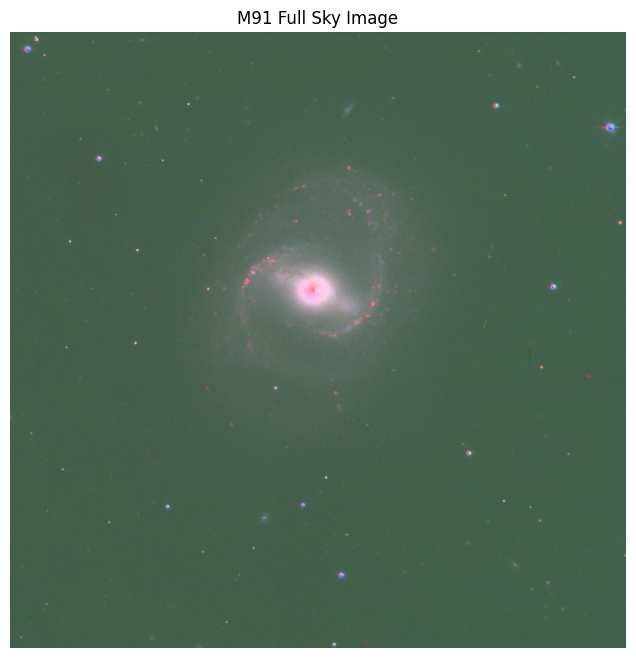
\includegraphics[width=.8\linewidth]{m91_fullsky.png}
    \caption{Full sky image including the M91 Galaxy}
    \label{fig:1}
\end{figure}

In \autoref{fig:2}, the M91 is zoomed-in on, capturing the spiral arms and the bar across, as well as effectively capturing the redder and brighter H$\upalpha$ areas within the centre of mass (COM) and the ends of the arms. A series of images for different stretch and Q values were plotted for comparison and analysis in \autoref{fig:A4} in the \hyperref[sec:A]{Appendix}. The images shown here use a stretch of 2 and a Q value of 0.5.

\begin{figure}[ht]
    \centering
    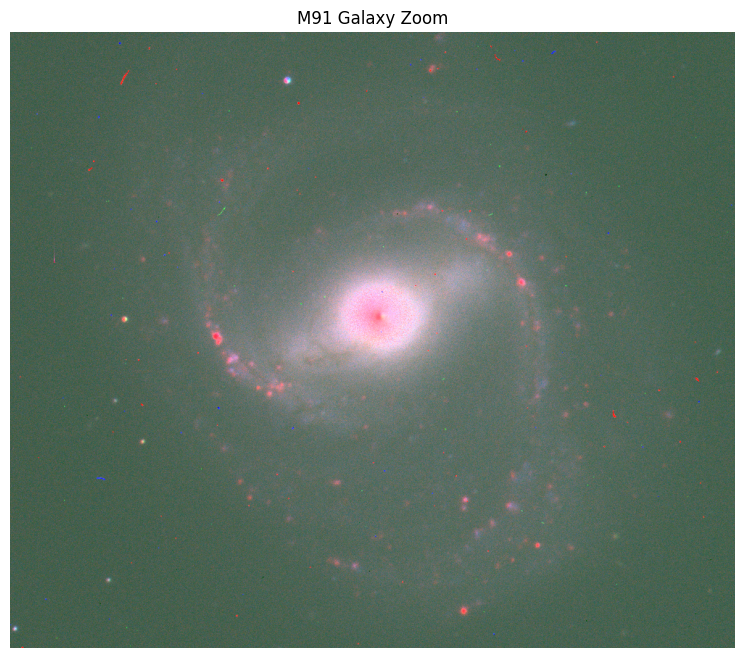
\includegraphics[width=.8\linewidth]{m91_galaxy.png}
    \caption{Zoomed-in image of the M91 Galaxy}
    \label{fig:2}
\end{figure}

\subsection{NN Serpentis}

The masterbias image (\autoref{fig:A5.1}) and masterflat image for the clear filter (\autoref{fig:A5.2}) for the NN Ser are shown in the \hyperref[sec:A]{Appendix}, the masterflat having a normalisation factor of approximately 1.000.

From the file list containing 18 FITS files for imaging, one was chosen as the reference image. This image was reduced as before, and the sources were found and plotted using the \verb|DAOStarFinder|. By increasing or decreasing the threshold, more or less sources would be found and plotted respectively. A reasonable value was chosen such that the function would not mistake background sky noise as a point source. The sources found are shown in \autoref{fig:3}. With direct comparison to a reference image with the stars labelled, the position of the NN Ser and surrounding reference stars was found as the following: \#40: A, \#48: B, \#47: C, \#26: D, \# 39: NN Ser. Due to a zeropoint much different than the other reference stars, reference star D was omitted from calculations.

\begin{figure}[H]
    \centering
    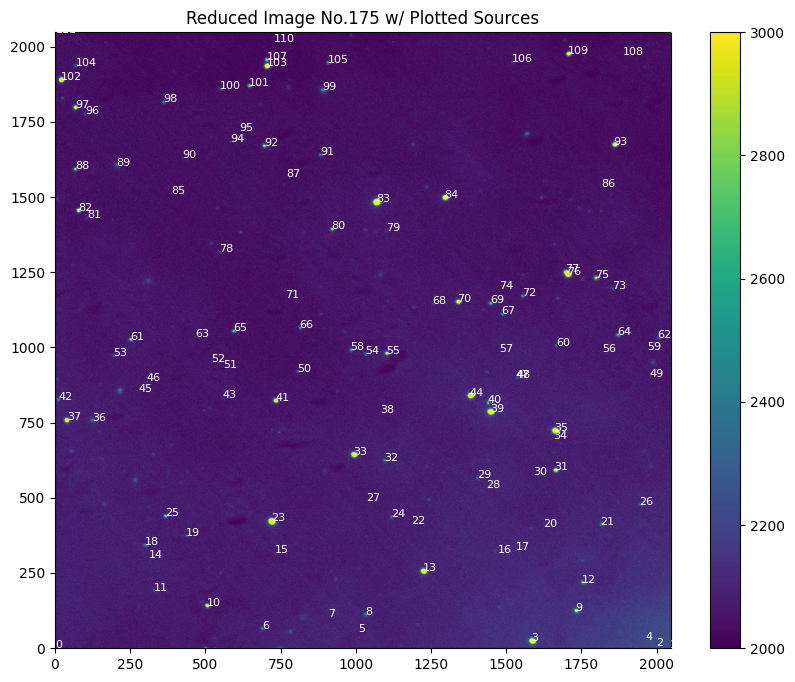
\includegraphics[width=.95\linewidth]{nnser_refimage.png}
    \caption{Reference image from the file list from which the reference star and NN Ser positions were extracted: \#40: A, \#48: B, \#47: C, \#26: D, \# 39: NN Ser}
    \label{fig:3}
\end{figure}

With a loop that located the same stars on the other 17 images based on the locations of the stars in the initial reference image shown in \autoref{fig:A6}, the zeropoints for the reference stars were found and used to calculate the magnitude for the NN Ser in each image, shown in \autoref{tab:1}. With these values, the lightcurve shown in \autoref{fig:4} was plotted. The red downwards-pointing triangle indicate the calculated limiting magnitudes for when the NN Ser was eclipsing, the magnitudes of which are shown in the highlighted yellow cells in \autoref{tab:1} in the \hyperref[sec:A]{Appendix}.

\begin{figure}[H]
    \centering
    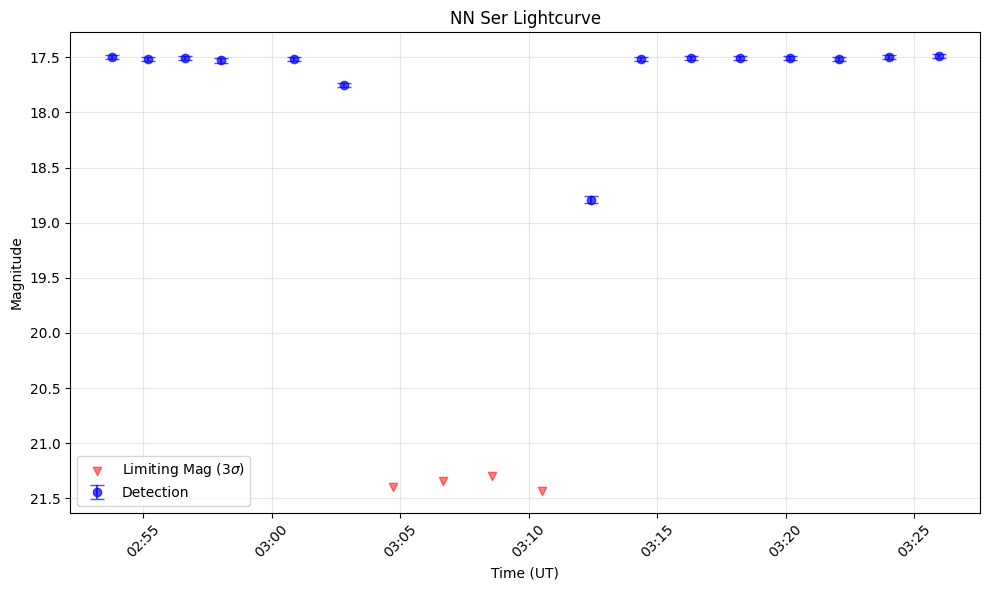
\includegraphics[width=\linewidth]{nnser_lightcurve.png}
    \caption{Lightcurve for the NN Ser from the magnitudes found using }
    \label{fig:4}
\end{figure}

\subsubsection{TESS Data}

A file containing the information of the NN Ser binary system taken by TESS was also provided. The information contained within it was used to plot a periodogram (top) of the Lomb-Scargle power against the period, of which the best period for the eclipsing binary was shown with a dotted red line at approximately 0.13 days, and a phase-folded lightcurve (bottom) in \autoref{fig:5}.

\begin{figure}[H]
    \centering
    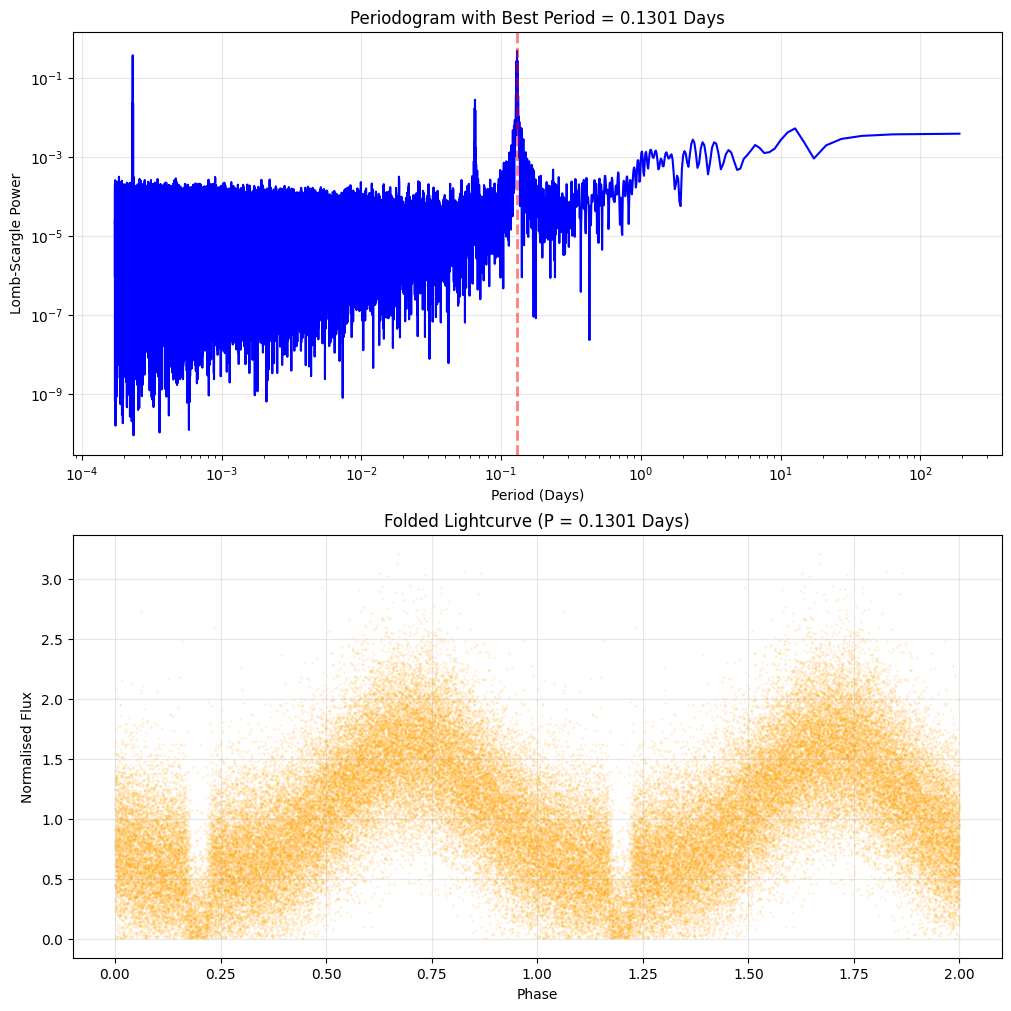
\includegraphics[width=\linewidth]{nnser_tessdata.png}
    \caption{NN Ser data from TESS plotted as a periodogram (top) and phase-folded lightcurve (bottom).}
    \label{fig:5}
\end{figure}

\section{Analysis and Discussion} \label{sec:4}

\subsection{Messier 91}

The first part of the experiment for the M91 images focused on reducing the raw CCD frames. The generated masterbias in \autoref{fig:A1} showed that the electronic noise floor and variations remained mostly constant for the duration of all bias captures, and the masterflat images for the three filters in \autoref{fig:A2} showed significant vignetting and several donut-shaped rings.

The application of these corrected frames, the masterbias and normalised masterflat images, corrected the variations in the pixels and signal-to-noise ratio for final object images. In these images, seen in \autoref{fig:A3}, the M91 is clearly and visually identified as a barred spiral galaxy, with its prominent central bar and bright central nucleus.

The appearance of the galaxy varies greatly across the three filters used as each filter captures a different wavelength range of light, which is indicative of a star's surface temperature; hotter stars appear bluer while cooler stars appear redder. The \textbf{blue (B)} filter shows the regions of highest energies and temperatures, therefore shortest wavelengths. With regards to the M91 galaxy, the effects of this filter would be most visible at the broader regions of the spiralling arms where new stars are most likely being actively formed. The \textbf{red (H$\mathbf{\upalpha}$)} filter shows the region of lowest energies and temperatures, therefore longest wavelengths. For the M91 galaxy, it best shows the older stars that are formed at the ends of the bar, and the central large nucleus as red light most efficiently penetrates interstellar dust and gas clouds. The \textbf{green (V)} filter captures the range of wavelengths between the other filters, called the \textit{visual} filter as it is the closest to the range of light we predominantly see with the naked eye.

These filter images were then combined into one composite RGB image, seen in \autoref{fig:1}, \autoref{fig:2}, and \autoref{fig:A4}, and the resulting colours show a map of the galaxy's evolution. A concentration of stars can be seen in the core and bar with the near-white light, indicating a multitude of different ages of stars, the redder stars where the bar and spiral arms connect indicate older stars while the bluer-tinged ends of the arms indicate recent stellar births.

Errors in this analysis and images primarily arise from the choosing and balancing of the "seeing" conditions, particularly when generating the colour composite image as a good balance between contrast and softening can be difficult to obtain, which can lead to finer details getting lost. Some error may have also arisen from the original capturing of the images too as some chromatic aberration, or at least improper alignment of the colour filters, can be seen in the colour composite images, most noticeably towards the outer edges.

\subsection{NN Serpentis}

The first part of the experiment for the NN Ser images were similar to the M91's, with a proper calibration of the masterbias and normalised masterflat, shown in \autoref{fig:A5}, in order to ensure that standard errors in equipment, like electronic noise and vignetting, are accounted for. The multiple images plotted for the NN Ser PCEB system are shown in \autoref{fig:A6} with the calculated and associated magnitudes of the NN Ser, including the zeropoints for the reference stars used, shown in \autoref{tab:1}. For this, reference star 'D' which is found in the reference material was omitted due to differing zeropoint values (D $\sim$28).

With these values a lightcurve for this system was plotted, seen in \autoref{fig:4}. This lightcurve shows a deep, sharp dip where there is a primary eclipse, indicating the white dwarf primary is eclipsed by the cooler red dwarf secondary companion.

Comparing this data with the data given by the TESS satellite observations, seen in \autoref{fig:5}. In the periodoram (top), we see the largest and clearest peak at around 0.13 days, which is the orbital period of the NN Ser. A difference is seen between both methods of capture, where the effects of the cooler star of the primary are with the peaks in the bottom graph where luminosity and therefore magnitude increase due to increased heating. The eclipsing dips are still seen in this graph, appearing as sharp and deep dips similarly to the lightcurve generated with the ground-based data. Error in data may appear from choosing an aperture size too small or too large, which differs what the program qualifies as a source.

There is a discrepancy in the magnitudes measured with the provided data, finding that a value of approximately 17.5 was achieved where the SIMBAD database states that the r' calibrated magnitude for the NN Ser is approximately 16.7 \cite{2000A&AS..143....9W}. The value obtained through calculations is approximately 0.8 magnitudes fainter than the reported value. Discrepancies may arise from errors in choosing the correct positions of the reference stars or atmospheric effects, or ineffective settings.

\section{Conclusion}

The generated colour composite RGB image of the M91 galaxy effectively demonstrated the theoretical principles covered of it being a barred spiral galaxy as well as a truncated anemic one. By isolating different wavelength bands, the B filter highlights regions of recent stellar births at the ends of the spiral arms that are blue-tinged, signalling the presence of hot, high energy stars. Contrarily, the H$\upalpha$ filter penetrated the interstellar dust and gas better, revealing older, cooler stars near the central nucleus and bar. This aligns perfectly with what had been described about the M91 being an anemic SB(rs)b(A) galaxy, as the lack of widespread star formation across the extended disk reflect the gas deficiency that had been discussed and expected, caused by the ram-pressure stripping within the Virgo Cluster.

Similarly, the photometric analysis of the NN Serpentis binary system showed successfully its classification as a PCEB. The generated lightcurves both from the ground-based data and the TESS satellite displayed the expected sharp and deep dips of the expected behaviour of the white dwarf primary being eclipsed by the cooler red dwarf secondary. Furthermore, an orbital period of approximately 0.13 days was observed from this data, matching the well-documented expected results. Although the magnitude for the NN Ser was using the ground-based data was calculated to be approximately 17.5, which is 0.8 magnitudes dimmer than expected 16.7 based on the SIMBAD database, which may be attributed to atmospheric effects, aperture sizing discrepancies, or ineffective settings. The distinct eclipsing behaviour remains present and observable in the plotted data, as expected.

%%%%%%%%%%%%%%%%%%%%

% References - switch to single column
\onecolumn

\bibliographystyle{IEEEtran}
\bibliography{PHYC30170References} \label{sec:ref}

\newpage

% Appendix - single column
\section*{Appendix} \label{sec:A}
\addcontentsline{toc}{section}{Appendix}

\subsection*{Figures}
\addcontentsline{toc}{subsection}{Figures}

\begin{figure}[H]
    \centering
    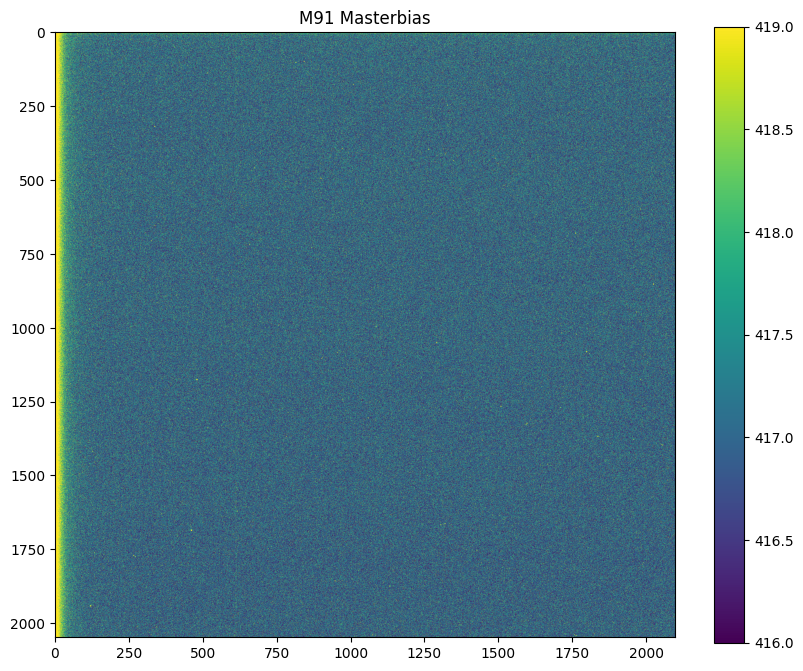
\includegraphics[width=.45\textwidth]{m91_masterbias.png}
    \caption{M91 Masterbias}
    \label{fig:A1}
\end{figure}

\begin{figure}[H]
    \centering
    \begin{subfigure}{.32\textwidth}
        \centering
        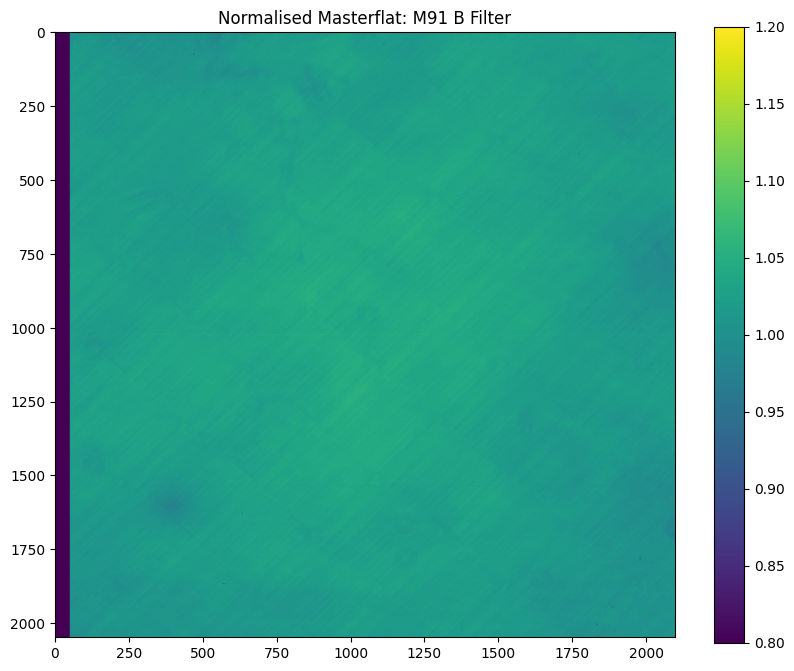
\includegraphics[width=\linewidth]{m91_Bmasterflat.png}
        \subcaption{B Filter}
        \label{fig:A2.1}
    \end{subfigure}
    \begin{subfigure}{.32\textwidth}
        \centering
        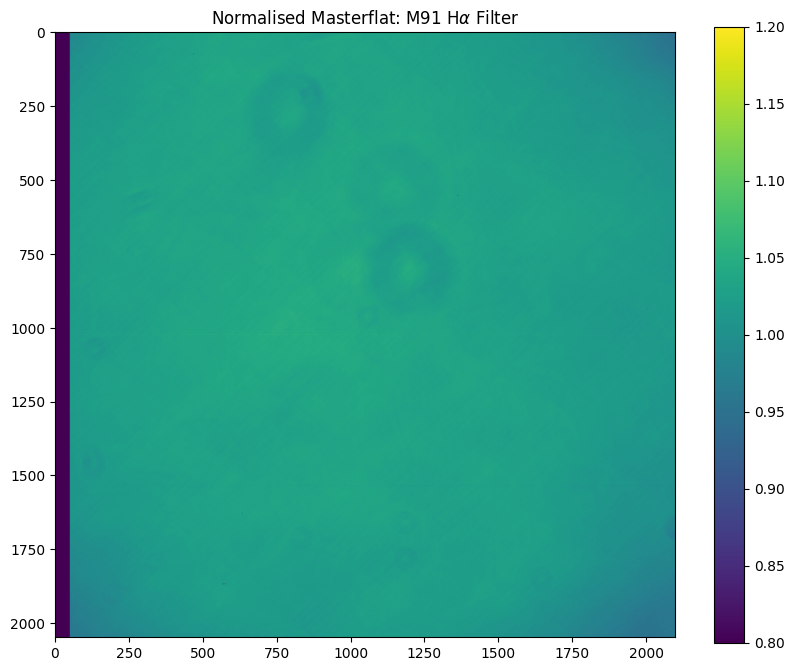
\includegraphics[width=\linewidth]{m91_HAmasterflat.png}
        \subcaption{H$\upalpha$ Filter}
        \label{fig:A2.2}
    \end{subfigure}
    \begin{subfigure}{.32\textwidth}
        \centering
        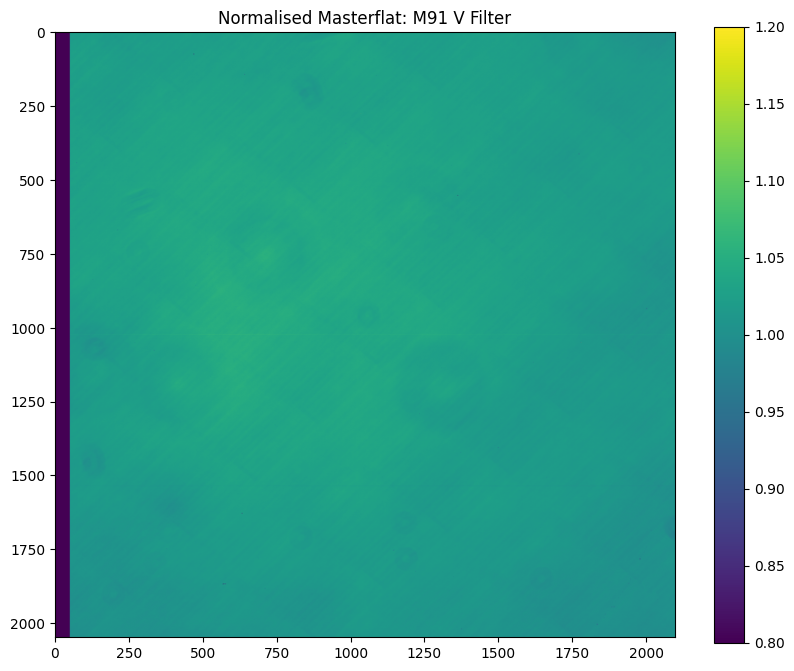
\includegraphics[width=\linewidth]{m91_Vmasterflat.png}
        \subcaption{V Filter}
        \label{fig:A2.3}
    \end{subfigure}
    \caption{M91 Masterflat for the (\subref{fig:A2.1}) B filter, (\subref{fig:A2.2}) H$\upalpha$ filter, (\subref{fig:A2.3}) V filter.}
    \label{fig:A2}
\end{figure}

\begin{figure}[H]
    \centering
    \begin{subfigure}{.32\textwidth}
        \centering
        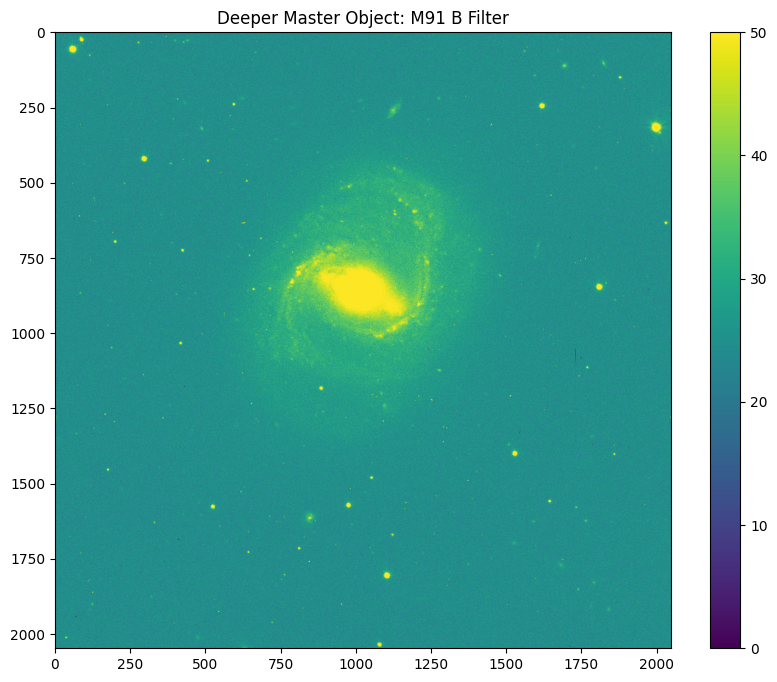
\includegraphics[width=\linewidth]{m91_Bdeeper.png}
        \subcaption{B Filter}
        \label{fig:A3.1}
    \end{subfigure}
    \begin{subfigure}{.32\textwidth}
        \centering
        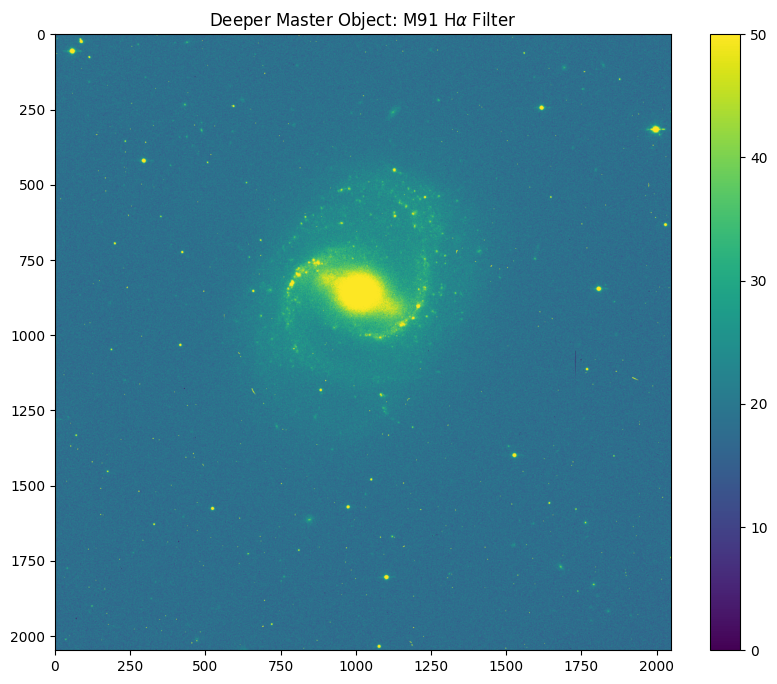
\includegraphics[width=\linewidth]{m91_HAdeeper.png}
        \subcaption{H$\upalpha$ Filter}
        \label{fig:A3.2}
    \end{subfigure}
    \begin{subfigure}{.32\textwidth}
        \centering
        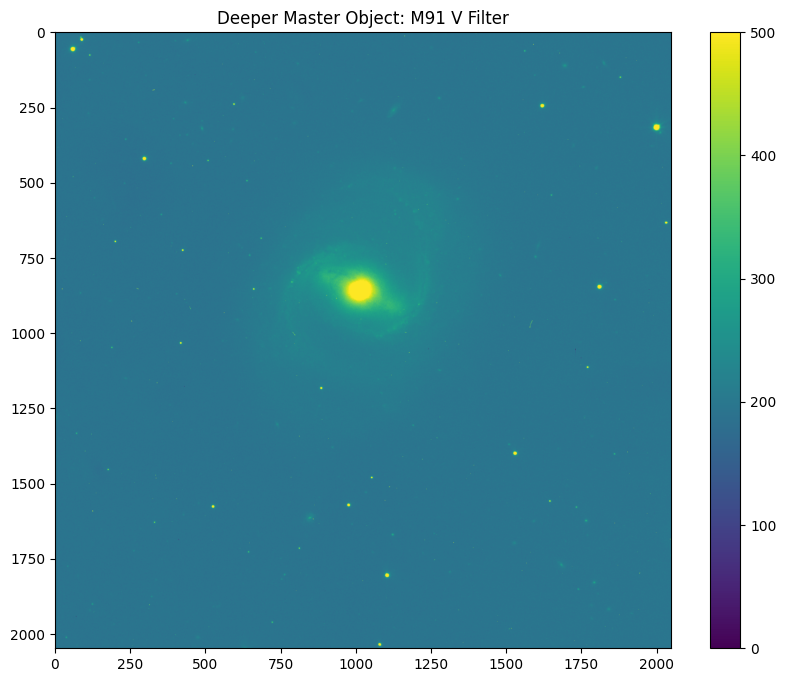
\includegraphics[width=\linewidth]{m91_Vdeeper.png}
        \subcaption{V Filter}
        \label{fig:A3.3}
    \end{subfigure}
    \caption{M91 deeper image for the (\subref{fig:A3.1}) B filter, (\subref{fig:A3.2}) H$\upalpha$ filter, (\subref{fig:A3.3}) V filter.}
    \label{fig:A3}
\end{figure}

\begin{figure}[H]
    \centering
    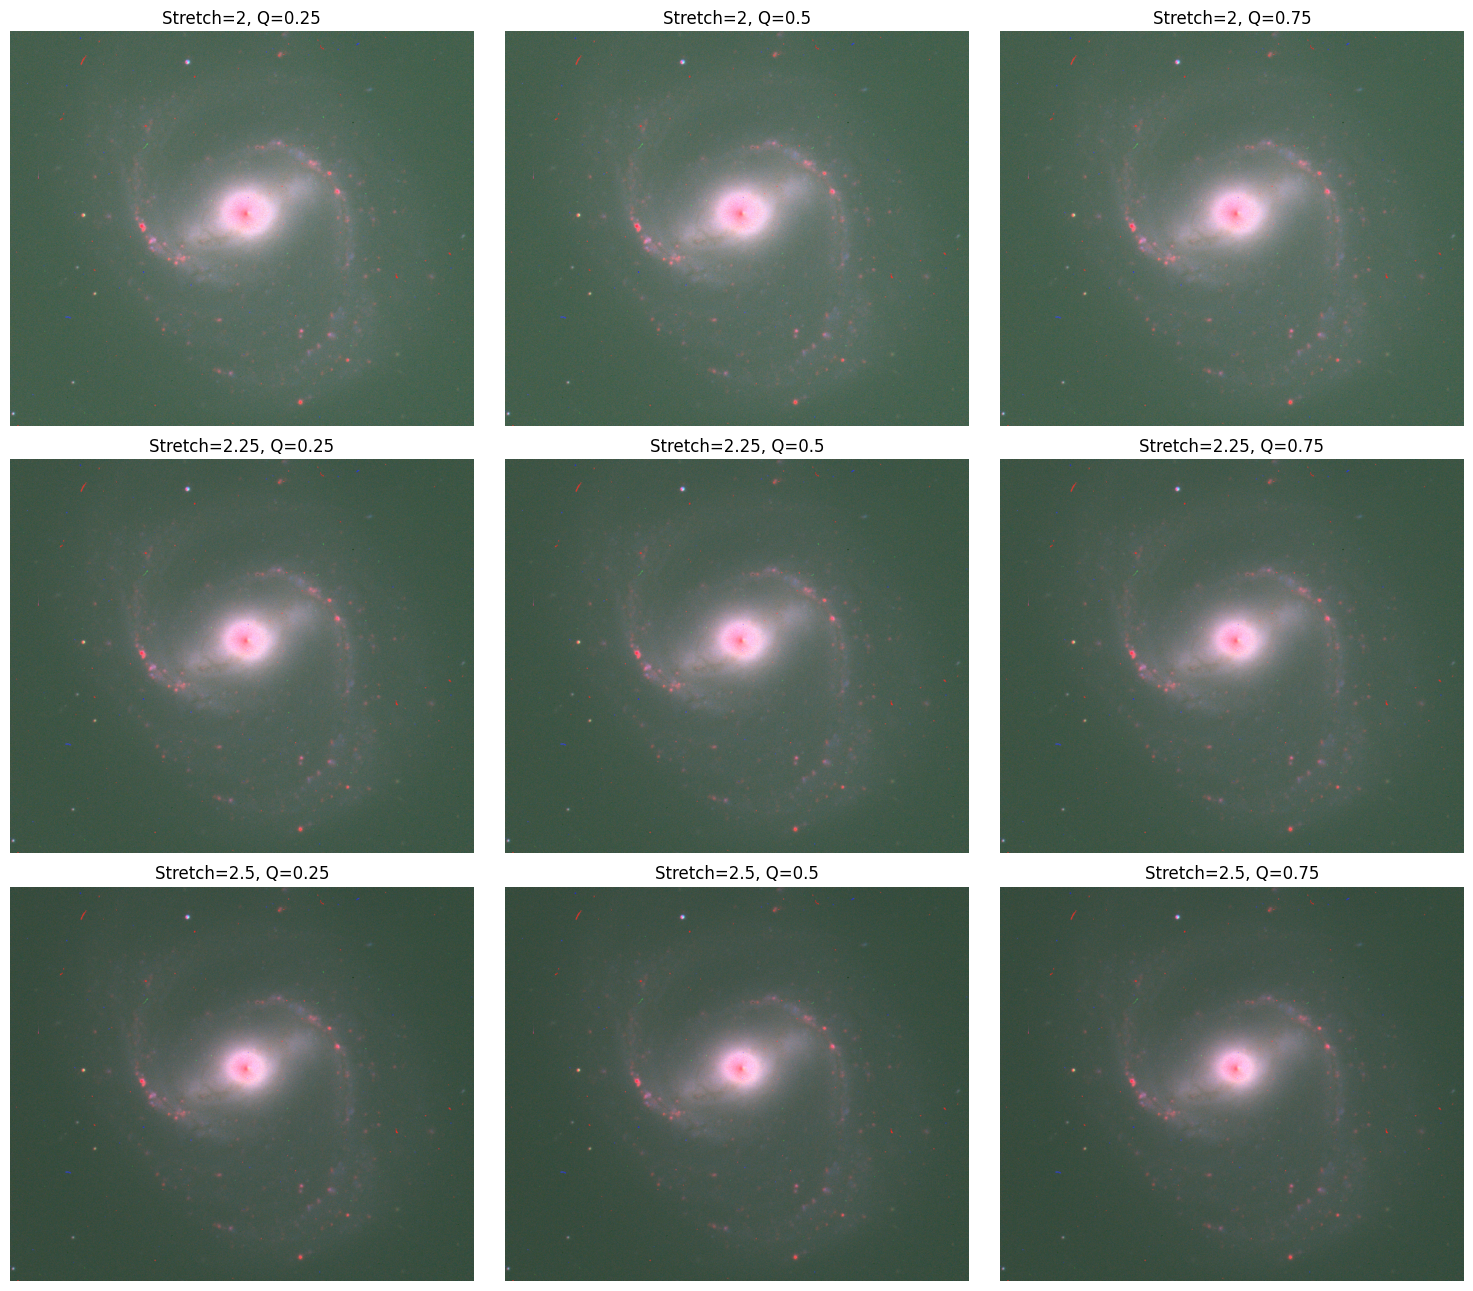
\includegraphics[width=\textwidth]{test_m91_galaxy.png}
    \caption{Full test of different stretch and Q values for the M91 Galaxy images.}
    \label{fig:A4}
\end{figure}

\begin{figure}[H]
    \centering
    \begin{subfigure}{.45\textwidth}
        \centering
        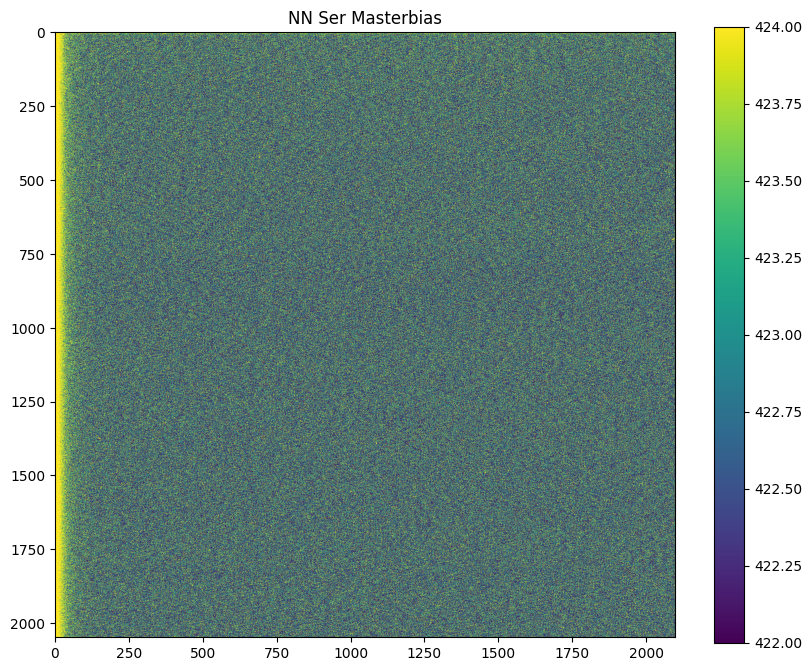
\includegraphics[width=\linewidth]{nnser_masterbias.png}
        \subcaption{Masterbias}
        \label{fig:A5.1}       
    \end{subfigure}
    \begin{subfigure}{.45\textwidth}
        \centering
        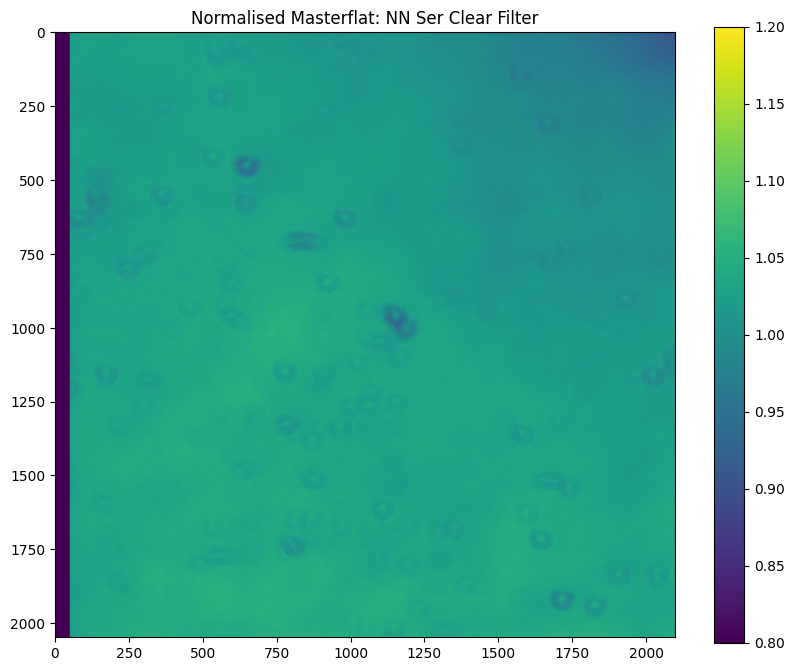
\includegraphics[width=\linewidth]{nnser_masterflat.png}
        \subcaption{Masterflat}
        \label{fig:A5.2}
    \end{subfigure}
    \caption{NN Ser (\subref{fig:A5.1}) Masterbias and (\subref{fig:A5.2}) Masterflat (clear filter) images.}
    \label{fig:A5}
\end{figure}

\begin{figure}[H]
    \centering
    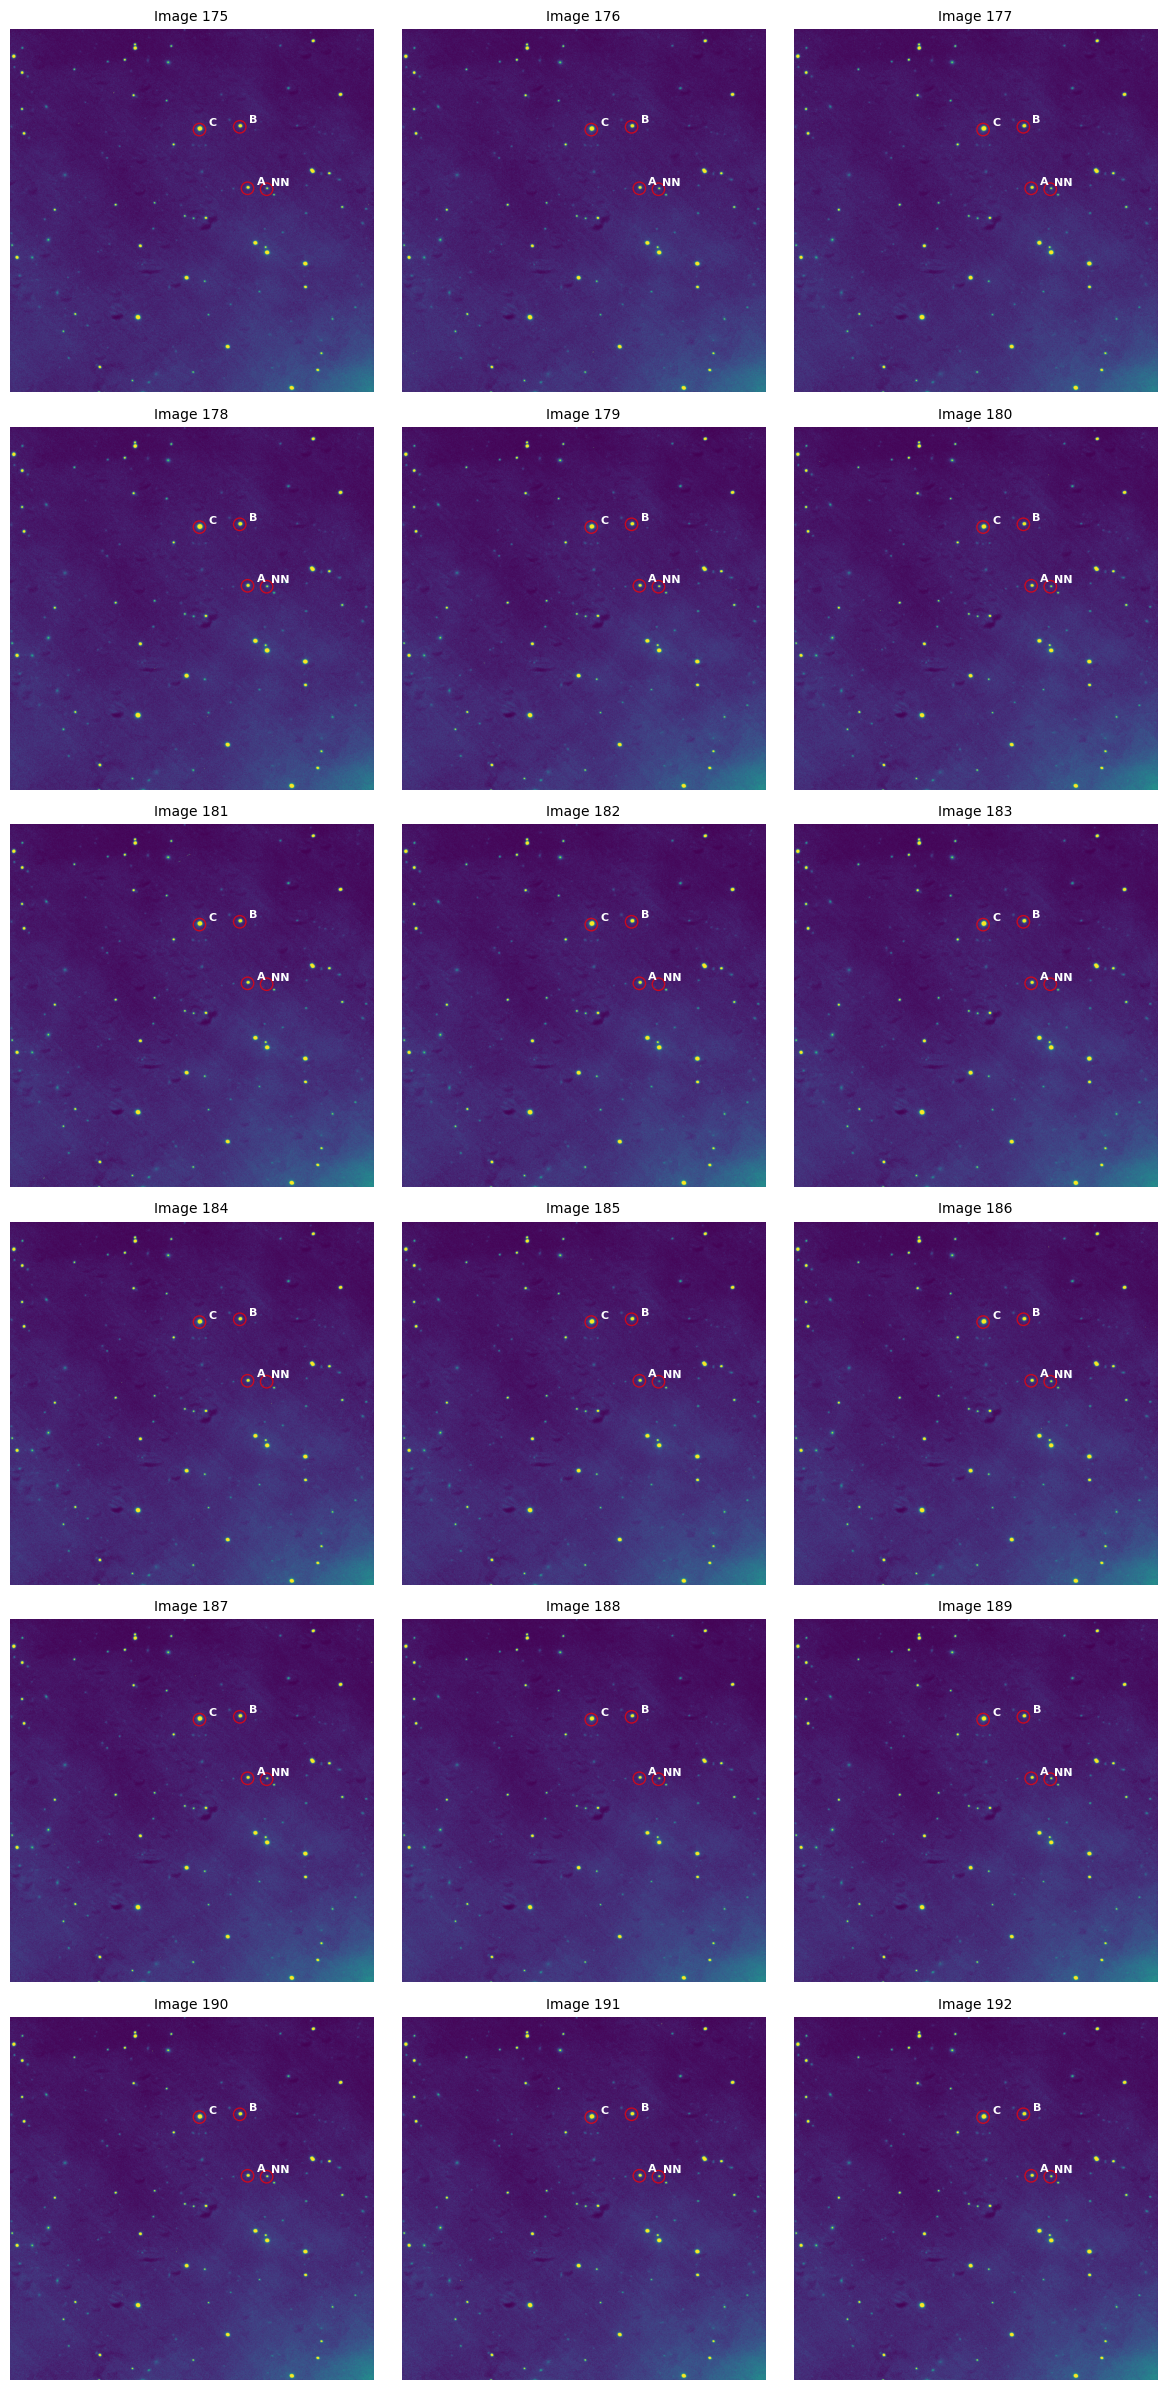
\includegraphics[width=.72\textwidth]{nnser_ALLreducedimgs.png}
    \caption{All reduced NN Ser images with NN Ser and reference stars labelled.}
    \label{fig:A6}
\end{figure}

\newpage

\subsection*{Tables}
\addcontentsline{toc}{subsection}{Tables}

\begin{table}[H]
\centering
\caption{Magnitude values for the NN Ser and the zeropoints for the A, B, C reference stars, with the limiting magnitudes highlighted in yellow.}
\label{tab:1}
\begin{tabular}{|
>{\columncolor[HTML]{C0C0C0}}c |c|c|c|c|}
\hline
\textbf{ID}  & \cellcolor[HTML]{C0C0C0}\textbf{Magnitude} & \cellcolor[HTML]{C0C0C0}\textbf{ZP (A)} & \cellcolor[HTML]{C0C0C0}\textbf{ZP (B)} & \cellcolor[HTML]{C0C0C0}\textbf{ZP (C)} \\ \hline
\textbf{175} & 17.498 ± 0.019                             & 29.163                                  & 29.201                                  & 29.219                                  \\ \hline
\textbf{176} & 17.516 ± 0.020                             & 29.172                                  & 29.207                                  & 29.234                                  \\ \hline
\textbf{177} & 17.507 ± 0.017                             & 29.118                                  & 29.145                                  & 29.158                                  \\ \hline
\textbf{178} & 17.527 ± 0.020                             & 29.010                                  & 29.046                                  & 29.065                                  \\ \hline
\textbf{179} & 17.519 ± 0.017                             & 29.661                                  & 29.697                                  & 29.718                                  \\ \hline
\textbf{180} & 17.754 ± 0.019                             & 29.673                                  & 29.710                                  & 29.731                                  \\ \hline
\textbf{181} & \cellcolor[HTML]{FFFE65}21.399             & 29.633                                  & 29.667                                  & 29.685                                  \\ \hline
\textbf{182} & \cellcolor[HTML]{FFFE65}21.342             & 29.560                                  & 29.595                                  & 29.624                                  \\ \hline
\textbf{183} & \cellcolor[HTML]{FFFE65}21.294             & 29.540                                  & 29.564                                  & 29.588                                  \\ \hline
\textbf{184} & \cellcolor[HTML]{FFFE65}21.432             & 29.660                                  & 29.697                                  & 29.719                                  \\ \hline
\textbf{185} & 18.791 ± 0.035                             & 29.637                                  & 29.672                                  & 29.691                                  \\ \hline
\textbf{186} & 17.515 ± 0.017                             & 29.614                                  & 29.651                                  & 29.673                                  \\ \hline
\textbf{187} & 17.505 ± 0.017                             & 29.635                                  & 29.673                                  & 29.692                                  \\ \hline
\textbf{188} & 17.504 ± 0.017                             & 29.661                                  & 29.693                                  & 29.717                                  \\ \hline
\textbf{189} & 17.503 ± 0.0.18                            & 29.692                                  & 29.730                                  & 29.753                                  \\ \hline
\textbf{190} & 17.517 ± 0.017                             & 29.711                                  & 29.745                                  & 29.773                                  \\ \hline
\textbf{191} & 17.500 ± 0.017                             & 29.699                                  & 29.731                                  & 29.761                                  \\ \hline
\textbf{192} & 17.489 ± 0.017                             & 29.669                                  & 29.701                                  & 29.728                                  \\ \hline
\end{tabular}
\end{table}

\includepdf[pages={1-3,6-7,12-13,15-25,29-31}]{/Users/JoanaUCD/Library/CloudStorage/OneDrive-UniversityCollegeDublin/Labs/labs-files/tex Files/astroimage.pdf}

\end{document}